\documentclass[unicode,aspectratio=43]{beamer}
\usetheme{Moscow}

\usepackage[utf8]{inputenc}
\usepackage[T2A]{fontenc}
\usepackage[main=russian,english]{babel}
\usepackage{tikz}

%%%%%%%%%%%%%%%%%%%%%%%%%%%%%%%%%%%%%%%%%%%%%%%%%%%%%%%%%
\def \ve{\varepsilon} % USE
\def \eps{\epsilon}
\def \del{\delta}
\def \ved{{\varepsilon,\del}}%
\def \KSD{\K^{\star, \delta}}
\def \lm{\lambda}
\def \Lm{\Lambda}
\def \la{\left\langle\rule{0pt}{3em}}
\def \ra{\right\rangle}
\def\mx{\mathsf m}
\def\fr{\mathsf f}
%%%%%%%%%%%%%%%%%%%%%%%%%%%%%%%%%%%%%%%%%%%%%%%%%%%%%%%%%
\newcommand{\Ab}[1]{(A.#1)}
%%%%%%%%%%%%%%%%%%%%%%%%%%%%%%%%%%%%%%%%%%%%%%%%%%%%%%%%%
\def\red{\textcolor{red}}
%%%%%%%%%%%%%%%%%%%%%%%%%%%%%%%%%%%%%%%%%%%%%%%%%%%%%%%%%
\def \gr{\nabla}
\def \pt{\partial}
\def \ptt{\partial_t}
\def \dv{\mbox{$\mbox{div}$}}
\def \div{{\rm div}\,}
%\def \to{\rightarrow}
\def \tow{\rightharpoonup}
%%%%%%%%%%%%%%%%%%%%%%%%%%%%%%%%%%%%%%%%%%%%%%%%%%%%%%%%%
\def \eqdef{\stackrel {\rm def} {=}}
\def \ds{\displaystyle}
%%%%%%%%%%%%%%%%%%%%%%%%%%%%%%%%%%%%%%%%%%%%%%%%%%%%%%%%%
\def \R{{\mathbb R}} \def \C{{\Bbb C}} \def \Z{{\Bbb Z}}
\def \I{{\Bbb I}} \def \N{{\Bbb N}} \def \K{{\mathbb K}}
\def \bs{\boldsymbol}
\def \fr{\mathsf f}
\def \ge{\mathfrak{g}}
%%%%%%%%%%%%%%%%%%%%%%%%%%%%%%%%%%%%%%%%%%%%%%%%%%%%%%%%%


\usepackage{amsmath,amssymb}

\hypersetup{
	pdfauthor={Vitaly Mazepov}
}

%\renewcommand{\thefootnote}{\fnsymbol{footnote}}
\usepackage{euler}
\usepackage{multirow}
\renewcommand*{\arraystretch}{1.2}

\graphicspath{{images/}}
\newcommand{\colorhref}[2]{\href{#1}{\textcolor{miptbase!30!black}{#2}}}

\newcounter{citenum}
\newcommand{\newtotcounter}[1]{}
%%% Реализация библиографии встроенными средствами посредством движка bibtex8 %%%

%%% Пакеты %%%
\usepackage{cite}                                   % Красивые ссылки на литературу


%%% Стили %%%
\bibliographystyle{../BibTeX-Styles/utf8gost71umod}    % Оформляем библиографию по ГОСТ 7.1 (ГОСТ Р 7.0.11-2011, 5.6.7)

\makeatletter
\renewcommand{\@biblabel}[1]{#1.}   % Заменяем библиографию с квадратных скобок на точку
\makeatother
%% Управление отступами между записями
%% требует etoolbox 
%% http://tex.stackexchange.com/a/105642
%\patchcmd\thebibliography
% {\labelsep}
% {\labelsep\itemsep=5pt\parsep=0pt\relax}
% {}
% {\typeout{Couldn't patch the command}}

%%% Цитирование %%%
\renewcommand\citepunct{;\penalty\citepunctpenalty%
    \hskip.13emplus.1emminus.1em\relax}                % Разделение ; при перечислении ссылок (ГОСТ Р 7.0.5-2008)


%%% Создание команд для вывода списка литературы %%%
\newcommand*{\insertbibliofull}{
\bibliography{../biblio/othercites,../biblio/authorpapersVAK,../biblio/authorpapers,../biblio/authorconferences}         % Подключаем BibTeX-базы % После запятых не должно быть лишних пробелов — он "думает", что это тоже имя пути
}

\newcommand*{\insertbiblioauthor}{
\bibliography{../biblio/authorpapersVAK,../biblio/authorpapers,../biblio/authorconferences}         % Подключаем BibTeX-базы % После запятых не должно быть лишних пробелов — он "думает", что это тоже имя пути
}

\newcommand*{\insertbiblioother}{
\bibliography{../biblio/othercites}         % Подключаем BibTeX-базы
}


%% Счётчик использованных ссылок на литературу, обрабатывающий с учётом неоднократных ссылок
%% Требуется дважды компилировать, поскольку ему нужно считать актуальный внешний файл со списком литературы
\newtotcounter{citenum}
\def\oldcite{}
\let\oldcite=\bibcite
\def\bibcite{\stepcounter{citenum}\oldcite}

\renewcommand{\citepunct}{,\,}

\title[Schlumberger]{}

\author[Мазепов Виталий]{\textbf{Мазепов Виталий}}

\newcommand{\Ip}{\mathrm{\mathit{I}}_\text{p}}
\renewcommand{\vec}[1]{\boldsymbol{\mathbf{#1}}}
\newcommand{\pd}[2]{\frac{\partial #1}{\partial #2}}
\let\dividesymbol\div
\renewcommand{\div}{\operatorname{div}}
\newcommand{\grad}{\operatorname{grad}}

\begin{document}

\begin{frame}[plain]

\tableofcontents
\end{frame}

\section{Резюме}

\begin{frame}\frametitle{Краткая информация}
	\scriptsize{
		Мазепов Виталий Александрович \\
		студент 5 курса факультета управления и прикладной математики МФТИ \\ 
		mazepov@phystech.edu \\
		+7(906)759 49 45 \\
		\small\textbf{Опыт} \\
		\scriptsize
		\begin{itemize}
			\item инженер 1 категории, лаборатория флюидодинамики и сейсмоакустики МФТИ - 2016 -- наст время
			\item техник, лаборатория флюидодинамики и сейсмоакустики МФТИ - 2015 -- 2016
		\end{itemize}
		\small\textbf{Исследования и профессиональные знания} \\
		\scriptsize
		\begin{itemize}
			\item июль 2016 -- наст время - магистерский диплом "Высокоточные алгоритмы численного моделирования распространения упругих волн в неоднородных средах"
			\item сентябрь 2015 -- июнь 2016 - бакалаврский диплом "Численное моделирование течения жидкости в трещиновато-пористых коллекторах"
		\end{itemize}
				\small\textbf{Навыки} \\
				\scriptsize
				\begin{itemize}
					\item Python (NumPy, SciPy, MatPlotLib)
					\item C/C++ (OpenMP, MPI)
					\item Matlab
				\end{itemize}
	}
\end{frame}

\section{Бакалаврский диплом}

\subsection{Постановка задачи}

\begin{frame}\frametitle{Постановка задачи}
\begin{columns}
\begin{column}{.5\textwidth}
Рассматриваем пористую среду, которая состоит из двух подобластей:
\begin{itemize}
\item Система плохо проницаемых блоков.
\item Система хорошо проницаемых трещин.
\end{itemize}
Среда - периодическая. 

$$
\ve = \frac{\ell}{L} \ll 1,
$$
где $\ell$ --- длина периода, а $L$ --- размер макроскопической области. 
\end{column}
\begin{column}{.4\textwidth}
\begin{figure}[ht!]
\centering
\begin{tikzpicture}[scale=0.7]
\def\rectanglepath{-- ++(1.3cm,0cm)  -- ++(0cm,1.3cm) -- ++(-1.3cm,0cm) -- cycle}

\filldraw[fill=white!30] (-0.1,-0.1) -- (5.9,-0.1)
                                         --  (5.9, 5.9) -- (-0.1, 5.9) -- cycle;

\filldraw[fill=lightgray] (0,  0) \rectanglepath;
\filldraw[fill=lightgray] (1.5,0) \rectanglepath;
\filldraw[fill=lightgray] (3,  0) \rectanglepath;
\filldraw[fill=lightgray] (4.5,0) \rectanglepath;

\filldraw[fill=lightgray] (0,  1.5) \rectanglepath;
\filldraw[fill=lightgray] (1.5,1.5) \rectanglepath;
\filldraw[fill=lightgray] (3,  1.5) \rectanglepath;
\filldraw[fill=lightgray] (4.5,1.5) \rectanglepath;

\filldraw[fill=lightgray] (0,  3.0) \rectanglepath;
\filldraw[fill=lightgray] (1.5,3.0) \rectanglepath;
\filldraw[fill=lightgray] (3,  3.0) \rectanglepath;
\filldraw[fill=lightgray] (4.5,3.0) \rectanglepath;

\filldraw[fill=lightgray] (0,  4.5) \rectanglepath;
\filldraw[fill=lightgray] (1.5,4.5) \rectanglepath;
\filldraw[fill=lightgray] (3,  4.5) \rectanglepath;
\filldraw[fill=lightgray] (4.5,4.5) \rectanglepath;

\draw (1.4,6.0)--(1.4,6.3);
\draw (2.9,6.0)--(2.9,6.3);
\draw[<->] (1.4,6.15)--(2.9,6.15);
\draw (2.2,6.4) node {$\ell$};

\draw[<->] (-0.1,-0.3)--(5.9,-0.3);
\draw (2.9,-0.65) node {$L$};

\draw (-0.4,5.9)--(-0.2,5.9);
\draw (-0.4,4.4)--(-0.2,4.4);
\draw[<->] (-0.3,4.4)--(-0.3,5.9);
\draw (-0.45,5.15) node {$\ell$};

\end{tikzpicture}

\caption{Периодическая область с трещинами и блоками.}

\end{figure}
\end{column}
\end{columns}

\end{frame}

\subsection{Результаты}

\begin{frame}\frametitle{Результаты численного моделирования}

\begin{figure}[ht!]
\centering
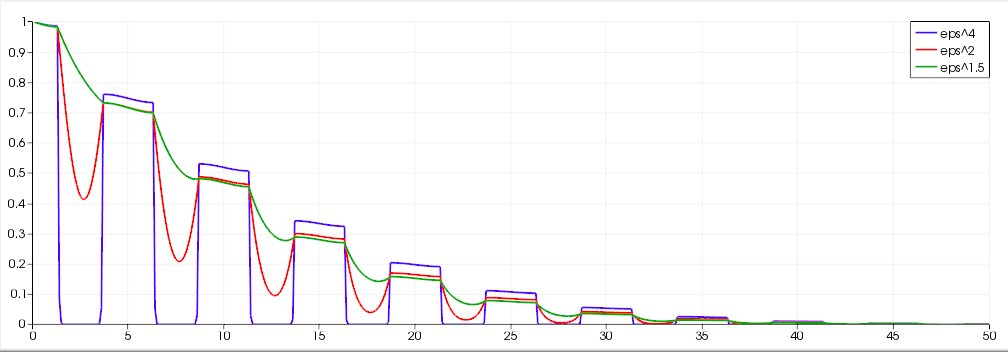
\includegraphics[scale=0.33]{voloshin2.jpg}
\caption{Давление жидкости в тонком слое для различных степеней контраста (сечение $y = 0$)}
\label{Figure 3}	
\end{figure}


\end{frame}

\begin{frame}\frametitle{Давление жидкости в тонком слое для различных значений параметра $\ve$}
\begin{figure}
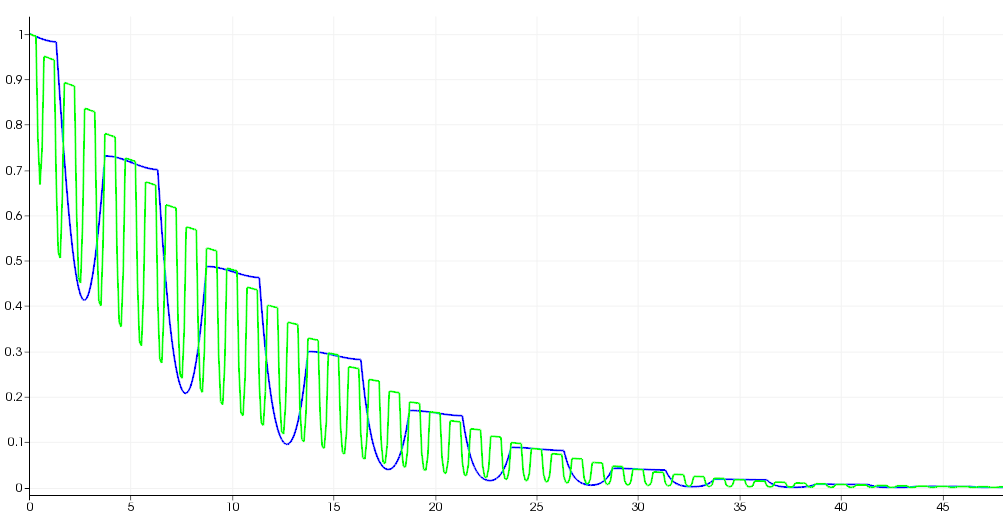
\includegraphics[scale=0.25]{voloshin3+.png}
\caption{Давление жидкости в момент времени $t = 1\, \ \text{мин}$ для $\ve = 0.05$ --- синяя кривая, $\ve = 0.01$ --- зеленая кривая}
\label{Figure 4}	
\end{figure}

\end{frame}

\subsection{Заключение}

\begin{frame}\frametitle{Заключение и выводы}
\begin{itemize}
\item В ходе работы создана программа, позволяющая моделировать однофазное течение слабосжимаемой жидкости в среде двойной пористости.
\item Проведены расчеты при различных значениях степени контраста $n$ и разных значениях параметра $\ve$:
\begin{itemize} 
\item Показано влияние степени контраста на характер течения в матричных блоках
\item Показана сходимость к предельному решению при $\ve \to 0$.
\end{itemize} 
\end{itemize}
\end{frame}

\section{Сверточные нейронные сети}

\begin{frame}{Сверточные сети}
	Сверточная нейронная сеть (англ. convolutional neural network, CNN) — архитектура искусственных нейронных сетей, нацеленная на распознавание изображений. 
	\begin{itemize} 
		\item Слой свертки (англ. convolution layer)
		\item Слой ReLU (англ. rectified linear unit) 
		\item Слой пулинга (англ. subsampling layer или англ. pooling layer)
	\end{itemize}
	Классическая архитектура выглядит следующим образом: 
	
	$Input \rightarrow  ReLU \rightarrow Conv \rightarrow ReLU \rightarrow Pool \rightarrow ReLU \rightarrow Fully Connected$
\end{frame}

\begin{frame}{Сверточный слой}
	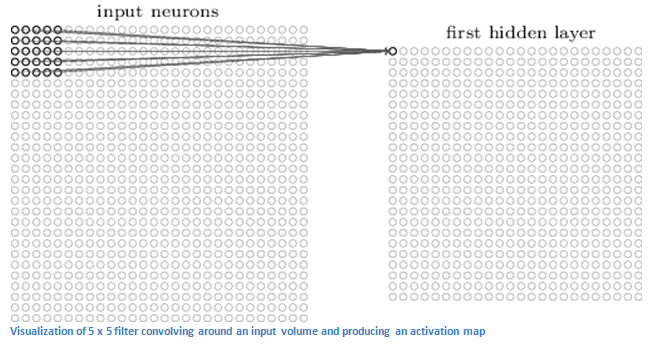
\includegraphics[scale=0.5]{1}
\end{frame}

\begin{frame}{Сверточный слой, пример}
	\begin{columns}
		\begin{column}{.5\textwidth}
			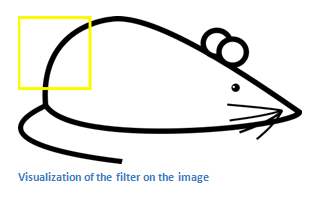
\includegraphics[scale=0.5]{3}
		\end{column}
		\begin{column}{.5\textwidth}
			При применении фильтра (поэлементное умножение и последующее сложение) к выделенной области получается относительно большое число. 
		\end{column}
	\end{columns}
	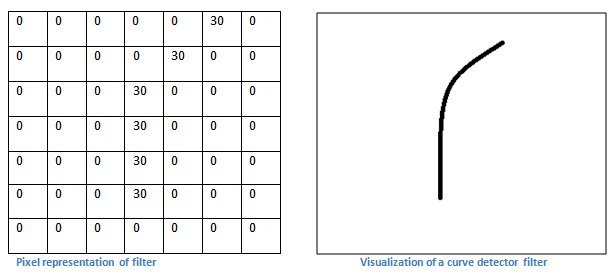
\includegraphics[scale=0.4]{2}
\end{frame}

\begin{frame}{Пулинг}
		\begin{columns}
			\begin{column}{.5\textwidth}
				\includegraphics[scale=0.55]{max_pooling.png}
			\end{column}
			\begin{column}{.5\textwidth}
				\begin{itemize}
					\item существенное уменьшение объема изображения
					\item факт наличия признака важнее его координат
					\item гарантия от переобучения за счет фильтрации ненужных деталей
				\end{itemize}
			\end{column}
		\end{columns}
\end{frame}

\begin{frame}{Обучение}
	Метод обратного распространения ошибки
	\begin{itemize}
		\item прямое распространение
		\item функция потери
		\item обратное распространение
		\item обновление веса
	\end{itemize}
	
	Минимизация функции потери осуществляется поправками весов с помощью, например, стохастического градиентного спуска. 
\end{frame}


\begin{frame}[plain]
  \begin{center}
  {\Huge Спасибо за внимание!}
  \vspace{8ex}

  Мазепов Виталий

  e-mail: \colorhref{mailto:mazepov@phystech.edu}{mazepov@phystech.edu}
  \end{center}
\end{frame}


\end{document}
